\begin{Exercise}[title=Chute d'échelle]
  $O_x$ est un sol horizontale et $Oy$ un mur vertical. Une échelle verticale $AB$ de masse $m$, de longueur $L=2l$ et de moment d'inertie par rapport à l'axe $Oz: J_\Delta =\frac{1}{3}mL^2$ évolue dans le plan de la figure Initialement elle est verticale et cet équilibre instable est détruit de façon infinitésimale, ce qui signifie que sa vitesse initiale est quasi nulle.
  \begin{center}
    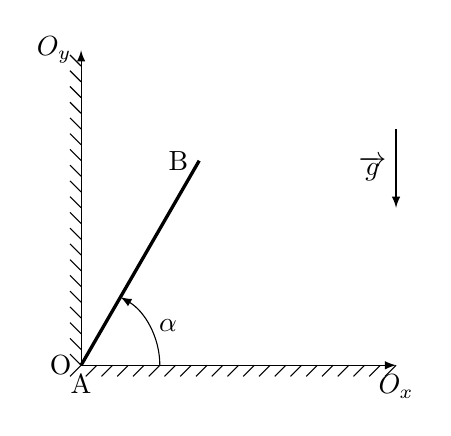
\begin{tikzpicture}
      \draw[-latex] (0,0) node[left]{O} -- ++(4,0) node[below]{$O_x$};
      \draw[-latex] (0,0) node[below]{A} -- ++(0,4) node[left]{$O_y$};
      \draw[decorate,decoration={border,amplitude=-0.2cm,segment length=0.2cm}] (0,0) --(4,0);
      \draw[decorate,decoration={border,amplitude=0.2cm,segment length=0.2cm}] (0,0) --(0,4);
      \draw[very thick] (0,0) -- ++(60:3)node[left]{B};
      \draw[-latex] (1,0) arc(0:60:1) node[midway,right]{$\alpha$};
      \draw[-latex] (4,3) -- (4,2)node[midway,left]{$\overrightarrow{g}$};
    \end{tikzpicture}
  \end{center}
  
	L'extrémité $A$ peut tourner librement en $O$ sans frottement.
	\Question Déterminer les expressions de $\dot{\alpha},\ddot{\alpha}$ en fonction de $g,l,\alpha$.
	\Question Calculer tant que $A$ est en $O$, les composantes $R_x$ et $R_y$ de la force de contact s'exerçant sur la tige; commentaires.
\end{Exercise}
\begin{Answer}
	\Question on a $\dd{}{t}\left(\frac{1}{3}m(2l)^2\dot{\alpha}\right) = -mgl\cos \alpha \implies \boxed{\ddot{\alpha} = \frac{-3g}{4l}\cos\alpha}$
On intègre apres mulitplication de la dérivée : $\dot{\alpha}^2=\frac{3g}{2l}(1-\sin\alpha)$
On peux aussi faire par l'énergie mécanique.
	\Question TRD en $G$
	$ \begin{cases}
	m\ddot{x} =R_x \\
	m\ddot{y} =R_y-mg
	\end{cases} $ de plus $\begin{cases}
	\ddot{x} = -l(\ddot{\alpha}\sin\alpha +\dot{\alpha}^2\cos\alpha)\\
	\ddot{y} = l(\ddot{\alpha}\cos\alpha +\dot{\alpha}^2\sin\alpha)\\
	\end{cases}$ \\
	donc :
	\[ \boxed{R_x = \frac{9}{4}mg\cos\alpha\left(\sin\alpha -\frac{2}{3}\right)} ~ ~ \boxed{R_y= \frac{1}{4}mg\left(3\sin\alpha-1\right)^2} \]
\end{Answer}
